\documentclass{standalone}
\usepackage{ tikz }
\usepackage{ xparse }
\usepackage{ amssymb }
\usepackage{../../macros}

\begin{document}
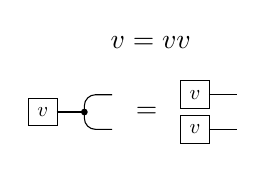
\begin{tikzpicture}[yscale=-1,x=1em,y=1.25em]

    \node at (3.4,-2) {$v \seq \fork = v \tensor v$};

    \node [draw, minimum width=1em, minimum height=1em] at (-0.5,0) {\scalebox{0.75}{$v$}};
    \draw (0,0) -- (1,0);
    \filldraw (1,0) circle (1pt);
    \draw [rounded corners]  (1,0) -- (1,-0.5) -- (2,-0.5);
    \draw [rounded corners]  (1,0) -- (1,0.5) -- (2,0.5);

    \node at (3.25,0) {$=$};

    \node [draw, minimum width=1em, minimum height=1em] at (5,-0.5) {\scalebox{0.75}{$v$}};
    \node [draw, minimum width=1em, minimum height=1em] at (5,0.5) {\scalebox{0.75}{$v$}};

    \draw (5.5,-0.5) -- (6.5,-0.5);
    \draw (5.5,0.5) -- (6.5,0.5);

\end{tikzpicture}
\end{document}